%%
%% This is file `Graphics_Guidelines.tex'
%% 
%% Copyright 2017 American Mathematical Society.
%% 
%% This file is part of the collection comprising the AMS Author Handbooks.
%% For details and license information, see the file README-AH.txt.
%%
%% The Current Maintainer of this work is the American Mathematical
%% Society.
%% 
%% ========================================================================
%% 

\chapter{Graphics}\label{ch:graphics}

\section{Getting started}

\noindent \textbf{Please take a moment to review the material in this
 chapter.} Problems with graphics in production can lead to significant
 delays in processing and publishing your work. Graphics are critically
 important in conveying large amounts of complex information and by
 observing a few relatively simple guidelines, you can assist in the
 efficiency of the publishing process.

\begin{itemize}
\item Use a standard \TeX\ graphics inclusion macro package.
 The recommended graphics inclusion package for \latexe/ is \pkg{graphicx}.
 Be sure that commands used to include graphics in \TeX\ are compatible
 with Radical Eye Software's dvips.
\item Do not place graphics for use in \TeX\ files in subdirectories.
\item Number figures consistently throughout the paper.
\item Use an in-text reference.
\item Set figure captions in \TeX.
\item Set figure captions below the figure.
\item Make sure figures are sized correctly and do not extend into the
  margins of the page.
\item Make sure that labels overlaid on a figure using a separate
  package do not extend beyond the space allotted to the figure.
\end{itemize}

\secwnote[ss:electronicgraphics]{File format}%
{The preferred file format for graphics is EPS (Encapsulated PostScript).\\
Other formats will be converted to EPS at the AMS.}

\begin{itemize}
\item Characteristics of EPS files can be checked by an automated
 procedure.  Individual features, e.g., the thickness of a rule, cannot
 be evaluated independently in a PDF graphic.
\end{itemize}

\secwnote[sec:resreq]{Resolution requirements for bitmap graphics}%
{Line art: 600 pixels per inch (PPI) at 100\%.\\
Halftone: 300 PPI at 100\%.\\
Combination halftone: 600 PPI at 100\%.}

\secwnote[sec:grsize]{Size of graphics}%
{Create graphics at 100\% of the size at which they will be printed.}

\begin{itemize}
\item If the figure is too large, resize the figure in a graphics program,
  not in \TeX.
\item This applies also to photographs (see section~\ref{sec:photo}).
\end{itemize}

\secwnote[sec:namef]{Naming files}%
{File names should be no longer than 20 alphanumeric characters. Do
  not use accented alphabetic characters. Avoid overly generic file
  names such as \fn{fig01.eps}.}

\secwnote[sec:placing]{Placing graphics in your document}%
{Use a standard \TeX\ graphics inclusion macro package.
We recommend \pkg{graphicx}.} 

\secwnote[sec:rules]{Lines and rules}%
{Do not use a line/rule weight less than half a point (.5 point) at 100\%.} 

\begin{itemize}
\item % Do not use a line/rule weight less than half a point (.5 point) at 100\%. 
 If you must scale your figure, be sure that you compensate by making line
 weights thicker.  A .5 point line scaled at 50\% becomes a .25 point line.
 Lines with weights less than half a point \emph{may} disappear during the
 printing process.
\item Increase graded lines in half-point increments
 (i.e., .5 point, 1 point, 1.5 points).  Otherwise, the lines will not
 appear as distinctly different lines.
\item Give lines that are a shade of gray (screened) or colored a line
  weight of at least 1 point at 100\%.  Gray and colored lines with weights
  less than 1 point look broken and jagged because of the small dot pattern
  used to simulate a shade of gray or color tone.
%\item For best results with graphics intended for online display, do not use a line/rule thinner than 1 point (1 pixel at 72 PPI) at 100\%.
%Although a .5 point line is acceptable for print, screen resolution is 72 PPI and a .5 point line will disappear online.
\end{itemize}

\secwnote[sec:gray]{Shades of gray (screens)}%
 {Screens (a pattern of small black and white dots used to simulate shades
  of gray) should not be lower than 10\% or higher than 85\%.}

\begin{itemize}
\item Screens outside the range 10\% to 85\% are either too light or too
 dark to print correctly.
\item Screen density should increase in increments of no less than 10\%.
 Screen variations of less than 10\% are not distinguishable.
\item Do not put (black or colored) type on a screen darker than 35\%.
 Type on a screen that is above 35\% is not legible.
\item White type can be used only on 100\% black.
 White type on a gray background looks broken and jagged because a small
 dot pattern is used to simulate shades of gray.
\end{itemize}

\secwnote[sec:fontu]{Font usage}%
{Fonts should be fully embedded in your graphics.} 

\begin{itemize}
\item Whenever possible, fonts used in graphics should match those used in text.
\item Fonts should be fully embedded in your graphics.
 If the fonts are not embedded in a graphic, it is possible that the font
 will be replaced with a default font such as Courier and the characters
 will not print properly. If you are unable to embed the fonts in your
 graphic, convert the fonts to paths (or outlines) prior to exporting the
 file to EPS\@.  The fonts can be converted in the program you used to create
 the graphics. (For assistance, consult your graphics program's
 documentation.)
\item Use Type 1 outline fonts instead of bitmap fonts.
 Type 1 outline fonts are vector based. These fonts do not lose quality
 when they are output to high-resolution printers.
\item Do not subset fonts included in your graphics.
 It is imperative that the full font set be included in every graphic. If
 only a subset of a font is included, a font error can occur, which may
 cause characters to disappear in both the graphic and the DVI file.
\item Avoid using fonts with city names such as Chicago, Monaco, Geneva, etc.
\end{itemize}

\needspace{4.5\baselineskip}

\secwnote[sec:multip]{Multiple-part figures}%
 {Multiple-part figures should be configured as one figure in a graphics
  program, not in \TeX.}

\begin{itemize}
\item Aligning multiple-part figures is very difficult in \TeX. It is
 easier and more cost-effective to do so in a graphics program.
\end{itemize}

\secwnote[sec:crop]{Cropping and bounding boxes}%
{Do not crop by pasting areas of white over portions of the graphic.}

\begin{itemize}
\item When using a smaller area of a larger graphic, clip or crop within
 the graphics application to delete all but the desired portion.
\item Do not crop by pasting areas of white over portions of the graphic.
 Doing this will make the bounding box larger than it should be and will
 cause problems when the graphic is included in \TeX.
\item If possible, verify that bounding box information is correct.
 If the bounding box is not correct, graphics might be clipped off in
 unexpected ways.
\end{itemize}

\ifmonograph
 \section{Color graphics}\label{sec:color}
\else
 \secwnote[sec:color]{Color graphics}%
 {Graphics submitted in color will appear in color in the online version of
 \ifmemoirs \Memos.
 \else dual products.
 \fi
 The print version will normally appear in black and white, except in
 special circumstances, when the
 \ifjournal Managing \fi
 Editor and Publisher mutually agree that color graphics are
 warranted. The AMS offers color to authors who are willing to pay for
 four-color graphics that aren't deemed essential to the mathematics
 by the Editor and Publisher.}
\fi

\subsection{Color spaces and gamuts}

\noindent There are two main color spaces in use: RGB (Red-Green-Blue)
and CMYK (Cyan-Magenta-Yellow-Black). The former is used for
light-emitting displays (computer monitors, for instance) while the
latter is used for printing. 

\marginpar{\noindent\lower1.25in\hbox{
\includegraphics[scale=0.5]{rgb-cmyk}}}

One of the characteristics of a color space, such as RGB or CMYK, is
its \emph{gamut}, the range of colors that it can reproduce. The RGB
color space has a much larger color gamut than the CMYK color space,
as shown in Figure~\ref{fig:gamuts} (page~\pageref{fig:gamuts}, left).
Colors in the RGB color space that lie outside the gamut of the CMYK
color space must be approximated by the CMYK color space, with varying
degrees of success: Figure~\ref{fig:gamuts} (page~\pageref{fig:gamuts},
right) compares the color output from various color technologies. CMYK
colors can generally appear more muted when compared to their RGB
counterparts. All RGB color graphics have to be converted to CMYK for
printing. All color graphics, both RGB and CMYK, are subjected to analysis
here at the AMS and optimized for printed publication.

\textbf{\emph{Above all, bear in mind that color graphics viewed on a
 monitor or printed on a personal printer will not necessarily be an
 accurate rendering of how colors will look when printed on a press.}}
 Our Graphic Arts group has years of experience in bringing out the best
 from a wide variety of graphics, particularly color graphics.

\begin{figure}
\noindent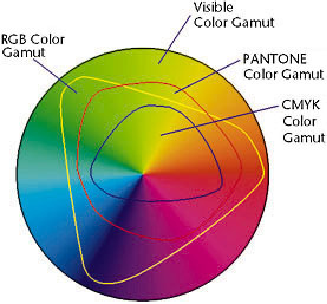
\includegraphics[width=0.4\textwidth]{gamuts}\qquad
\includegraphics[width=0.4\textwidth]{spectrum}
\caption{\emph{Left:} A comparison of the colors available in various color
  spaces. \emph{Right:} A comparison of the colors available with various
  display technologies.}\label{fig:gamuts}
\end{figure}
%% websupport1.citytech.cuny.edu/faculty/phenry/gamuts.html. Currently 'Not found'.

%Dual product (print and electronic) or print-only journals:  CMYK format.
%Electronic-only journals:  RGB format.  
%Books: CMYK format.

\subsection{Requirements for graphics to be published in color}

\textbf{Graphics intended to be printed in color should be submitted in
 CMYK format. If you submit RGB files they will be converted to CMYK\@.}
 The AMS cannot guarantee that color reproduction in the print product will
 match the RGB file.

\ifjournal
 For electronic-only journals \emph{only}, RGB files are preferred.
\fi

\subsection{Color graphics to be printed in black and white or
 grayscale\texorpdfstring{\nopunct\ \ignorespaces}{}}
%	Color graphics to be printed in black and white or grayscale
 \textbf{should be converted to black and white or grayscale before
 being submitted to the AMS\@.}
 When color graphics are printed in black and white or grayscale, sometimes
 lighter colors, such as yellow, disappear, or darker colors, such as red
 and blue, appear to be the same tone. It is preferable that you convert
 your color graphics to grayscale and check to be sure that all the
 elements in your graphics print as desired---see
%        Figure~\ref{fig2gray}, page~\pageref{fig2gray}. Check your
 Figure~\ref{fig2gray}, \vpageref[above]{fig2gray}. Check your color
 figures on a black and white printer to ensure that the black and white
 printout of your figure is legible.

\begin{figure}[t]

\includegraphics{Color2Gray}
\caption{Colors don't always have the intended effect when converted to grayscale.}
\label{fig2gray}
\end{figure}

\subsection{Shades of colors} Inherently light colors should be handled
 carefully when using shades of them. Whereas 50\% red turns out to be a
 usable pink, a 50\% yellow or cyan may be almost invisible.

\subsection{Colored lines\texorpdfstring{\nopunct}{}} should be no less
 than .5 point in width. Colored lines in inherently light colors
 (e.g. yellow and cyan) should always be at or near 100\% in tint.

\needspace{4.5\baselineskip}

\secwnote[sec:tsize]{Using type in graphics}%
 {Type within graphics requires special attention to reproduce legibly.}

\begin{itemize}
\item Basic type size should be no less than 10 point at 100\%.
 Although 10-point type is acceptable for print, for graphics intended
 to be viewed online, screen resolution is 72 PPI and 10-point type
 will be difficult to read.
\item Do not put type on a dark background. 
 Dark type on dark colors is not legible.
\item Check your color figures on a black and white printer to ensure that
 the black and white printout of your figure is legible.
\end{itemize}

\secwnote[sec:tables]{Tables}%
{Tables can be thought of as a special kind of graphic. They often require
 a great deal of attention to make them effective.}

\begin{itemize}

\item Make sure that the width of the table does not exceed the width of
 the text block.

\item Very wide tables can be rotated using the \pkg{rotating} package
 together with the \env{sidewaystable} environment. Remember that tables
 (and figures) should be rotated such that the left-hand side of the table
 (or figure), after rotation, is at the bottom of the page.

\item Set table captions above the table.

\item For more help on the formatting of tables, see \cite[chapter 5]{MG}
 and \cite{voss-tbl}.
\end{itemize}

\secwnote[sec:photo]{Photographs}%
{Photographs must be at a minimum resolution of 300 dpi at the actual size
 that the photograph will be printed in the published product.}

\begin{itemize}
\item Photographs should be at least 300 dpi in resolution at the actual
 size that the photograph will be printed in the published product.  Do
 not scale photographs in \TeX.
\item File format can be EPS, TIFF, or JPEG.
\item Color photographs must be saved in CMYK format. (See Color graphics,
 section~\ref{sec:color}.)
\end{itemize}

\section{\TeX\ graphics}

There are several ways of providing graphics by the use of \TeX\ coding,
the principal choices being

\begin{description}
\item[tikz]Based on the PGF (portable graphics format), this is a very
 flexible environment for creating graphics within a \TeX\ document. Note
 that it functions equally well in dvips-based \latex/ and \pdfLaTeX/ as
 well as the newer varieties of \TeX\ such as \XeLaTeX/ and \LuaLaTeX/.
 The native documentation \cite{tkz} is excellent, though massive. There
 are two very good primers by Mertz and Slough: \cite{MeSlp} and
 \cite{MeSlt}. A large set of examples, often generously documented, can be
 found at \cite{tkz-ex}.
\item[pstricks]Also a very flexible and useful environment for drawing in
 \TeX. It is most easily used with dvips-based \TeX, though, with some
 care, it can be used with \pdfLaTeX/. There is an excellent reference
 book by Herbert Voss, \emph{PSTricks: Graphics and PostScript for \TeX\
 and \latex/} \cite{voss-pst}. The use of pstricks is also covered in some
 detail in \cite[chapters five and six]{GM}.
\item[xy and xypic]Though generally associated with commutative diagrams,
 these packages can also serve as a general drawing environment for \TeX.
\end{description}
\noindent A great deal of general information about other \latex/ graphics
packages can be found in \cite{GM}.

\section{Using a package to apply labels to graphics}

Several packages exist whose purpose is to place labels on graphics.
Use of such a package does ensure consistent fonts.  However, labels
added by such a package do not modify the dimensions of a graphic,
whether it is an EPS file or a drawing prepared by other means.

If labels are applied outside the edges of the graphic, they can
extend into the margin on the sides, or above or below the graphic
into space intended to separate the page content from the running head,
or the graphic from a caption.  In extreme cases, they can overprint
surrounding material, with no warning being issued.  Authors using
such packages should be alert to this possibility, and carefully check
the graphics where such labeling has been used.

If it is not possible to position labels within the boundaries of a
graphic, extra space should be added with \cn{vspace} to compensate.

\endinput
